\chapter{2022:Mark Braverman}
\label{chap:braverman}
\begin{center}
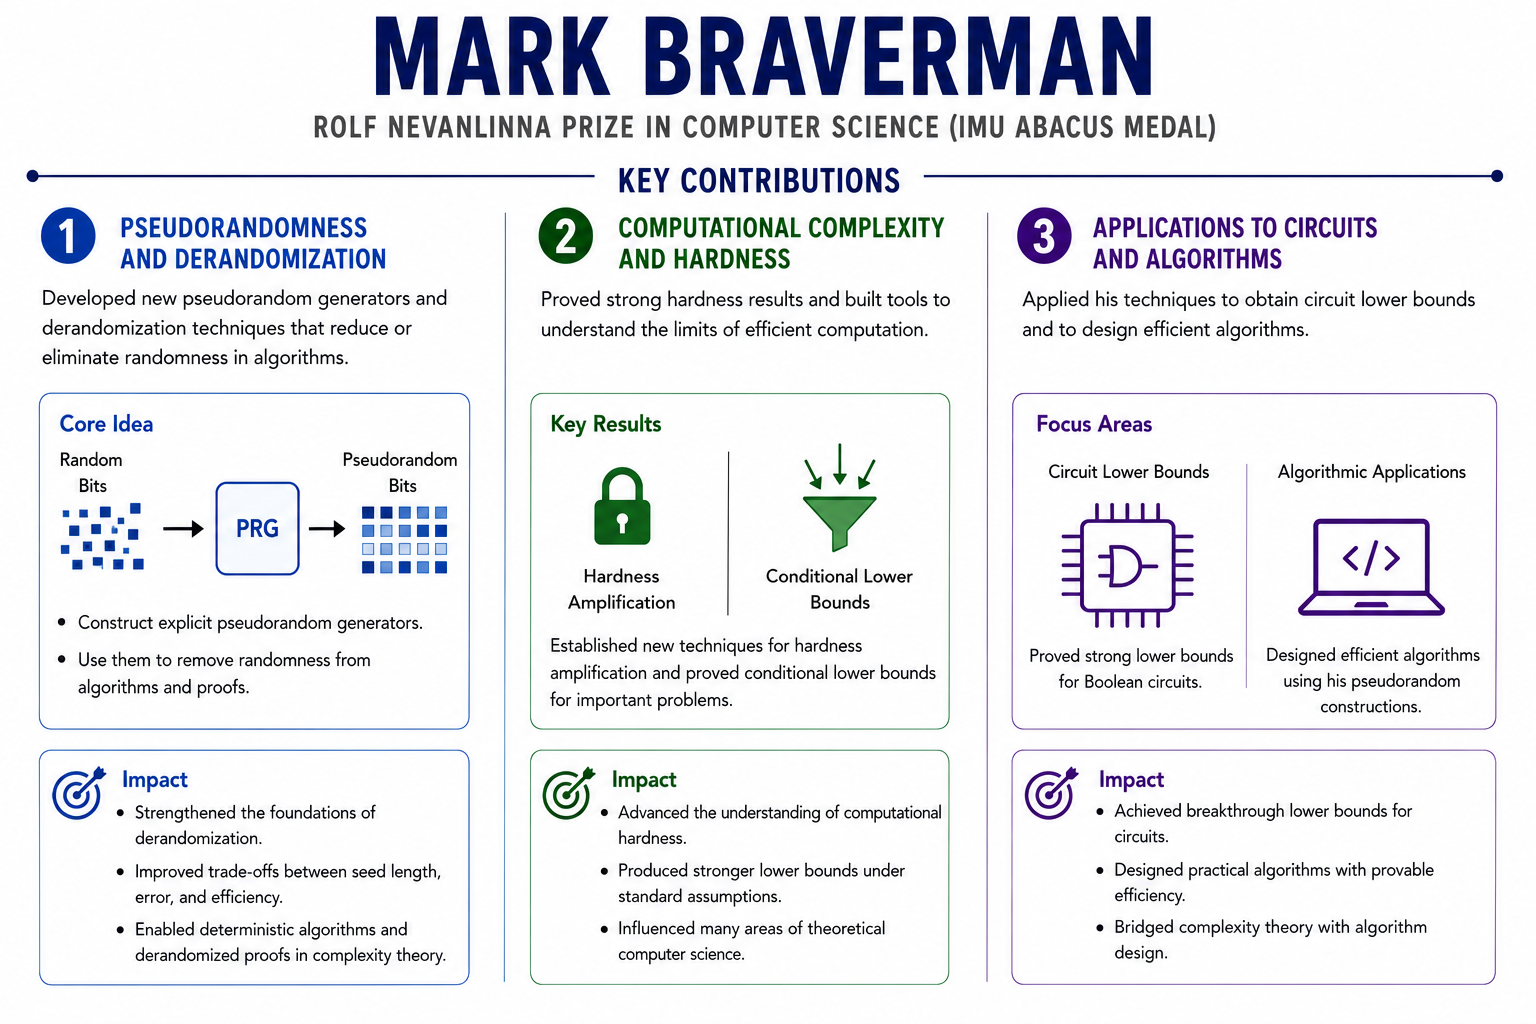
\includegraphics[width=\textwidth]{infographics/abacus11.png}
\end{center}
\normalchapterspacing
\index{Braverman, Mark}
\booknote{The central habit in this chapter is to ask not only what a protocol communicates, but what uncertainty it must destroy before the communication can succeed.}

\section{An Opening Story: The Party That Never Happened}
Two friends, Alice and Bob, sit in separate rooms planning a party. Each has privately decided whether they can come: a card reads ``0'' (no) or ``1'' (yes), and the party is worth planning only if \emph{both} cards read 1. They must agree on the answer, but every text message costs one coin, and they want to spend as few coins as possible. The obvious plan costs two coins: Alice texts her card, Bob texts his. But watch what actually happens. If Alice's card reads 0, the party is already off and Bob's answer changes nothing---the second coin buys nothing at all. The smarter plan is for Alice to text first and for Bob to text only if her card reads 1. Then two coins are needed only when her card reads 1, which happens half the time; on the other half, one coin settles everything.

Now suppose the pack is rigged so that 0-cards are ninety-nine times more common than 1-cards. The second message almost never matters, yet a worst-case budget of two coins still stands. A planner who pays typical costs spends a bit over one coin; an accountant who charges for \emph{information removed} rather than symbols sent demands only about a tenth of a coin. Three currencies, three prices for the same conversation. Deciding which price is honest, and learning to compute it, is the subject of this chapter---the work for which Mark Braverman received the 2022 Abacus Medal.

\section{The Problem}
Alice knows a private input $x$; Bob knows a private input $y$. By exchanging messages according to an agreed protocol, they must compute a function $f(x,y)$---for the party, ``do both cards read 1?''---correctly on every pair of inputs. The classical question is easy to state: how many bits must they exchange in the worst case? The deeper question is harder: what is each bit doing?

A transcript is not just a string; it is a sequence of decisions made under partial knowledge. Alice's message can reveal her card, rule out a whole class of worlds, coordinate a shared random experiment, or merely confirm an event Bob already believed. Counting symbols treats all four uses as equal, like pricing a house by counting its bricks. Two conversations of the same length can have radically different value: one message splits two equally likely worlds, another confirms a world already $99\%$ certain. The field's hardest open problems were about composition---must many independent copies cost many times one copy?---and about leakage: how much does a transcript reveal? Worst-case length could not answer either question.

So ``how many bits?'' and ``how much does the conversation buy?'' are different questions, and the party protocol is a microscope for the difference. The first message (Alice's card) always matters; the second (Bob's, sent half the time) matters only conditionally. A correct measure must charge them differently and let a long but nearly empty conversation cost almost nothing.

\section{The World Before}
Yao's 1979 model fixed the vocabulary: two players, private inputs, agreed rules, and a cost measured as the worst-case number of bits exchanged. The communication complexity $D(f)$ is the smallest worst-case length of any correct protocol, and the field built its power from lower-bound tools proving that specific functions genuinely need many bits.

Two tools dominated. A \emph{fooling set} is a collection of input pairs that all demand separate transcripts: if $(x,y)$ and $(x',y')$ both map to output 1 but the crossed pairs $(x,y')$ and $(x',y)$ map to 0, then no two of them can share a conversation, so the protocol needs at least as many distinct transcripts as the set has elements. The \emph{rank method} is more algebraic: write $f$ as a matrix with rows $x$, columns $y$, entries $f(x,y)$. Every deterministic protocol carves the matrix into monochromatic rectangles, one per transcript, and each rectangle is rank-1. A binary protocol of depth $t$ has at most $2^t$ transcripts, so $2^t$ is at least the matrix's rank. For equality of two $n$-bit strings the matrix is the $2^n\times 2^n$ identity, of rank $2^n$; hence at least $n$ bits are needed, and $n$ suffice. These tools are sharp, elegant, and measure only length.

The tools shared a blind spot: they could not explain why a long protocol might be nearly free. The party protocol has worst-case length 2 bits, yet on a typical conversation its second message is empty and even on the long branch it says one obvious thing; there was no vocabulary for ``this message was nearly predictable.'' Worst-case counting also could not amortize: for deterministic protocols $k$ copies trivially cost $k$ times one copy, but the honest average cost per copy over a stream of independent copies, where randomized protocols may share randomness, had no sharp answer---and neither did the question of how much information a transcript leaks about the inputs. A field built to answer ``how much must they say'' had no language for ``how much is revealed.''

The missing tool was a measure of communication that (i) decomposes round by round, (ii) adds over independent copies, and (iii) can be compared with transcript length. Information theory already had (i) and (ii) in entropy and the chain rule; the creative step was to point that machinery at interactive protocols and make the transcript itself the random variable being measured. The right unit of thought was not the symbol but the uncertainty destroyed.

\section{The New Idea}
The change of unit, in one sentence: charge a protocol for the information its transcript reveals about the inputs, not for the symbols it sends. A message the receiver could already predict is free; a message that splits the remaining uncertainty is expensive. This is the \emph{internal information cost} of the protocol,
\[
\operatorname{IC}_\mu(\Pi)=I(X;\Pi\mid Y)+I(Y;\Pi\mid X),
\]
where $\Pi$ is the random transcript and the conditioning records what each party already knows: Alice holds $X$, Bob holds $Y$, and information already sitting on its own side of the border is not charged for crossing it. (With public randomness $R$ shared by both, condition on $R$ too, since the shared coin is free.) The conditioning is not cosmetic: it is what makes the party protocol cost $3/2$ bits instead of $2$, as the worked example will show.

Three consequences follow from this unit.

\subsection{Compression: little information means few bits}
If a protocol reveals almost nothing, its transcript should be reproducible with almost no communication. From Bob's point of view, Alice's message is a sample from a distribution she can compute; with shared randomness, both players can search the random tape for that sample together, paying only for the part Bob could not have predicted. The compression principle states that a transcript of internal information cost $c$ can be simulated with communication proportional to $c$, up to overhead growing with rounds and error. Its sharpest form, Braverman--Rao's \emph{information equals amortized communication}, is an equality: the honest per-copy cost of many independent copies of a function is exactly the internal information cost of one copy.

\subsection{Direct sums: copies add up}
If one copy needs information $c$, then $k$ independent copies need $kc$. This direct-sum statement looks obvious and is the entire point: information, unlike worst-case length, satisfies the additivity amortized reasoning demands. Independent coordinates contribute independently to the transcript's information---the machinery is the chain rule. The subtlety is that conditioning on a whole transcript can couple coordinates that started independent; the fix is a random-coordinate embedding that converts the $k$-copy protocol into a one-copy protocol of the same per-copy cost.

\subsection{Noise: checkpoints and entangled correction}
Real channels flip bits, and one corrupted message changes the meaning of every later message: the parties may silently disagree about which history they share. Error correction cannot be bolted on beneath the computation, since the players may not even agree on what to correct. Robust interactive protocols must create checkpoints---frequent cheap confirmations that both parties stand on the same transcript---so computation and correction become entangled. In standard interactive-coding models with a fixed noise rate below the permitted threshold, Braverman and collaborators showed that a protocol of length $n$ can be simulated with only a constant-factor communication overhead and arbitrarily small error. The exact guarantee depends on the channel, noise rate, and feedback assumptions; the information viewpoint turned a believed polylogarithmic overhead into a constant.

\section{How It Works: Worked Examples}

\subsection{A warm-up: how much does a noisy coin flip tell us?}
Let $X$ be a fair bit, so $H(X)=1$. Suppose a friend tells us the value of $Z$, obtained by flipping $X$ with probability $p$: if $X=0$ then $Z=1$ with probability $p$; if $X=1$ then $Z=0$ with probability $p$. How much do we learn about $X$ by hearing $Z$?

Write $H(p)=-p\log_2 p-(1-p)\log_2(1-p)$ for the binary entropy function. Given $X$, the observation $Z$ is a coin flip with bias $p$, so $H(Z\mid X)=H(p)$. Meanwhile $Z$ is still a fair bit overall, because flipping a fair coin with probability $p$ leaves it fair: $H(Z)=1$. Therefore
\[
I(X;Z)=H(Z)-H(Z\mid X)=1-H(p).
\]
Check the endpoints. If $p=0$ then $H(0)=0$ and $I=1$: $Z$ always equals $X$, so hearing $Z$ reveals $X$ completely. If $p=1/2$ then $H(1/2)=1$ and $I=0$: $Z$ is a fresh fair coin flip, statistically independent of $X$. Now one interior value. For $p=1/4$,
\[
H(1/4)=-\tfrac14\log_2\tfrac14-\tfrac34\log_2\tfrac34=\tfrac12+\tfrac34(0.415)\approx 0.811,
\]
using $\log_2 4=2$ and $\log_2(3/4)=\log_2 3-2\approx -0.415$. So a $3/4$-reliable observation is worth $I(X;Z)\approx0.189$ bits---less than a fifth of a bit, because most of what it says was already predictable. That is the first concrete lesson of the chapter.

\subsection{The two-bit AND protocol: a conversation worth $3/2$ bits}
Return to the party. $X$ and $Y$ are independent fair bits, and the protocol is the smart one: Alice sends $X$; if $X=1$, Bob sends $Y$; if $X=0$, Bob sends nothing. The three possible transcripts and their probabilities are:
\begin{center}
\begin{tabular}{lcc}
\toprule
Transcript & Input & Probability \\
\midrule
``0'' & $X=0$ & $1/2$ \\
``1,0'' & $X=1$, $Y=0$ & $1/4$ \\
``1,1'' & $X=1$, $Y=1$ & $1/4$ \\
\bottomrule
\end{tabular}
\end{center}
Compute the internal information cost by hand, one term at a time.

\emph{Alice's contribution.} For $I(X;\Pi\mid Y)$, fix $Y=0$. Then $X$ is still a fair bit, so $H(X\mid Y=0)=1$, and the transcript determines $X$: ``0'' means $X=0$, ``1,0'' means $X=1$. Thus $H(X\mid \Pi,Y=0)=0$ and $I(X;\Pi\mid Y=0)=1$. The same with $Y=1$ gives $I(X;\Pi\mid Y=1)=1$, so averaging over $Y$,
\[
I(X;\Pi\mid Y)=\tfrac12\cdot 1+\tfrac12\cdot 1=1.
\]

\emph{Bob's contribution.} For $I(Y;\Pi\mid X)$, split by $X$. If $X=0$, the transcript is always ``0'' and says nothing about $Y$, contributing 0. If $X=1$, the transcript is ``1,Y'' and determines $Y$ exactly, contributing $H(Y\mid X=1)-0=1$. Averaging over $X$,
\[
I(Y;\Pi\mid X)=\tfrac12\cdot 0+\tfrac12\cdot 1=\tfrac12.
\]

The internal information cost is therefore $1+\tfrac12=\tfrac32$ bits, even though the worst-case transcript carries two symbols. The missing half-bit is Bob's message: worth a full bit when sent, it is sent only when $X=1$, so on average it contributes half a bit. A worst-case accountant charges 2 bits; the information accountant charges $3/2$. As a check, the transcript distribution $1/2,1/4,1/4$ has entropy $\tfrac12\cdot1+\tfrac14\cdot2+\tfrac14\cdot2=\tfrac32$ bits, so the external information cost $I(X,Y;\Pi)$ is also $3/2$ here.

Now the rigged pack: keep $Y$ fair but let $\Pr[X=0]=1-\delta$. Bob speaks with probability $\delta$ and then reveals $Y$ fully, so $I(Y;\Pi\mid X)=\delta$. For either fixed $Y$, Alice's message determines $X$, whose entropy is now $h(\delta)$ (the binary entropy of the biased bit), so $I(X;\Pi\mid Y)=h(\delta)$; the cost is $h(\delta)+\delta$. At $\delta=1/2$ this reproduces $\tfrac32$; at $\delta=1/4$ it is about $0.811+0.25\approx1.06$ bits; as $\delta\to0$ it tends to $0$ while the worst-case transcript still holds two symbols. Information and worst-case length are different currencies indeed.

\section{The Mathematics in Brief}
The quantities are few, and each is a compact record of an idea already met. The model, precisely: a \emph{deterministic protocol} for $f$ is a finite binary tree whose internal nodes alternate between the two players; at a node on the player's turn, a bit is sent whose value is a function of that player's input and the transcript so far, and each leaf is labeled by the answer. The \emph{communication complexity} $D(f)$ is the minimum, over correct protocols, of the worst-case depth. Every deterministic protocol of depth $t$ partitions the input matrix into at most $2^t$ monochromatic rectangles, one per transcript, and each rectangle is rank-1; the transcript count is therefore at least the rank of the matrix of $f$ (the \emph{rank method}), and at least the size of any fooling set. For a discrete random variable $X$ with probabilities $p_x$, the entropy is the expected surprise,
\[
H(X)=-\sum_x p_x\log_2 p_x,
\]
measured in bits. The conditional entropy
\[
H(X\mid Y)=\sum_y \PP(Y=y)\,H(X\mid Y=y)
\]
is the uncertainty about $X$ remaining after hearing $Y$, averaged over what $Y$ might say. The mutual information $I(X;Y)=H(X)-H(X\mid Y)$ is the reduction in that uncertainty, and it is symmetric. The chain rule
\[
H(X,Y)=H(X)+H(Y\mid X)
\]
is the algebraic reason everything decomposes: the entropy of a pair is the entropy of the first coordinate plus the conditional entropy of the second. Applied message by message to a transcript $\Pi=(M_1,\dots,M_r)$, it becomes
\[
I(X;\Pi\mid Y)=\sum_{i=1}^r I(X;M_i\mid Y,M_{<i}),
\]
charging each round exactly for the uncertainty that round removes, given everything already said.

The internal information cost of a protocol on input distribution $\mu$ is the quantity this chapter is about,
\[
\operatorname{IC}_\mu(\Pi)=I(X;\Pi\mid Y,R)+I(Y;\Pi\mid X,R),
\]
with $R$ the public randomness, free to both parties. The external information cost $I(X,Y;\Pi)$ instead measures what a third-party observer learns from the whole transcript---a question about leakage rather than negotiation. On top of these definitions stand two theorems. The \emph{compression} theorem says that a transcript of internal information cost $c$ can be simulated with communication roughly $c$ plus an overhead depending on rounds and error---little information, few bits. The \emph{direct-sum} theorem says that $k$ independent copies under the product distribution satisfy
\[
\operatorname{IC}_{\mu^k}(f^k)=k\,\operatorname{IC}_\mu(f):
\]
copies add exactly. Why? Independence makes the transcript's information decompose coordinate by coordinate through the chain rule; the caveat is that conditioning on a shared transcript can couple coordinates that started independent. The proof repairs this by embedding one copy into a random coordinate of the full protocol and averaging: a $k$-copy protocol, restricted to a randomly chosen coordinate, is a valid one-copy protocol of cost equal to the average per-coordinate cost. So one copy can never be cheaper than the average, and $k$ copies need at least $k$ times one copy. Information, unlike length, composes.

The sharpest form is an \emph{equality}, Braverman--Rao's \emph{information equals amortized communication}. Let $D^{\mathrm{pub}}_\mu(f^{\otimes k})$ be the communication cost of the best public-coin protocol computing $k$ independent copies of $f$ under the product distribution. Then
\[
\operatorname{IC}_\mu(f)=\lim_{k\to\infty}\frac{D^{\mathrm{pub}}_\mu(f^{\otimes k})}{k}.
\]
The upper bound (amortized cost is at most information) is compression: a transcript of internal information cost $c$ can be simulated with communication $\sim c$ plus overhead depending on rounds and error, so many copies can be handled at roughly their per-copy information. The lower bound is the direct sum above. Length has no such equality: worst-case length does not add under independent copies in any usable way, which is precisely why the field could not compute an honest per-copy price before information entered.

\section{Limits and Modern Views}
The framework is powerful and, like any measuring instrument, only as good as its calibration \cite{imu2022}. Information complexity is \emph{distributional}: every value is computed under a chosen input distribution, and choosing it is a creative act. A distributional lower bound transfers to a worst-case statement only with care, since a protocol may be cheap on typical inputs and expensive on rare ones, and approximate protocols need explicit error accounting because allowing error changes which uncertainty must be destroyed. Multiparty protocols spread information over many correlated views; quantum protocols replace messages with states whose measurement can destroy information; adaptive settings generate transcripts whose future questions depend on past answers. Each setting needs a refined notion, but the invariant survives: a constrained process must transform uncertainty into knowledge, and that transformation should compose under the operation being studied.

The framework also grew outward \cite{braverman15}. In \emph{streaming} algorithms, a small-space algorithm's answers about a long stream are a transcript in disguise, and communication lower bounds transfer to space through such embeddings. In \emph{data structures}, one encodes a communication problem into memory and query patterns; a too-cheap data structure would yield an implausibly cheap protocol, an approach used for lower bounds on extended formulations of linear programs \cite{braverman11}. In \emph{privacy}, the fields meet in the same object: differential privacy demands that transcript distributions under neighboring databases be hard to distinguish, and Pinsker's inequality
\[
\norm{P-Q}_{\mathrm{TV}}\le\sqrt{\frac{\ln 2}{2}\,D(P\Vert Q)}
\]
(for base-2 divergence) quantifies the bridge from small divergence to small distinguishing power. The lesson is to match the quantity to the guarantee: mutual information is an average while privacy is a worst case over neighbors, so low information does not automatically buy worst-case privacy \cite{braverman14}. Information complexity did not replace communication complexity; it changed the unit of thought, and that unit now circulates wherever a distributed computation must account for what it reveals.

\section{Exercises and Self-Study Guide}
\begin{enumerate}[label=\textbf{E\arabic*.}]
\item In the noisy-bit model, compute $I(X;Z)=1-H(p)$ for $p=1/3$ and $p=1/8$, and verify the endpoints $p=0$ and $p=1/2$ again from scratch.
\hint{Use $H(1/3)\approx0.918$ so $I\approx0.082$, and $H(1/8)\approx0.544$ so $I\approx0.456$; at $p=0$ the observation is exact, at $p=1/2$ it is a fresh fair flip.}
\item Two correlated bits have joint probabilities $\PP(0,0)=\PP(1,1)=3/8$ and $\PP(0,1)=\PP(1,0)=1/8$. Compute the marginals, $H(X)$, $H(Y)$, $H(X,Y)$, and $I(X;Y)$ directly from the joint table.
\hint{Both marginals are fair, so $H(X)=H(Y)=1$ and $H(X,Y)=2\cdot\tfrac38\log_2\tfrac83+2\cdot\tfrac18\log_2 8\approx1.811$; hence $I(X;Y)\approx0.189$ bits---the same number as the $p=1/4$ noisy bit, though the mechanism differs.}
\item Using the same joint table, verify the chain rule $H(X,Y)=H(X)+H(Y\mid X)$ by computing $H(Y\mid X=0)$ and $H(Y\mid X=1)$ and averaging.
\hint{Given $X=0$, $Y$ takes value 0 with probability $3/4$; both conditional entropies are $H(3/4)=H(1/4)\approx0.811$, so $H(Y\mid X)\approx0.811$ and the sum with $H(X)=1$ matches $H(X,Y)$.}
\item Design a public-coin protocol for equality of $n$-bit strings with error at most $1/8$. State precisely which distributional assumption, if any, your information calculation would need.
\hint{Both parties use public randomness to pick a hash $h$ from a 2-universal family into $\{0,1\}^3$ and compare $h(x)$ with $h(y)$; distinct strings collide with probability at most $1/8$. The correctness claim needs no input distribution, but any information-cost computation must fix one, e.g.\ uniform inputs.}
\item Take a one-round protocol in which Alice's message comes from a distribution that depends on her private input---say message ``1'' only when her input is exceptional, probability $\delta$---and attempt to compress it with shared randomness. Identify exactly where the simulation needs Alice's input.
\hint{Shared randomness can sample from a fixed distribution, but Alice's message distribution is conditional on her secret input. The simulator must know when to send the rare message, and describing that event costs about $\log_2(1/\delta)$ bits, which is the information the message really carries.}
\item Formulate a privacy-versus-computation question for a streaming algorithm: what plays the role of the transcript, and what would you charge?
\hint{Let the transcript be the sequence of query answers; charge for information about individual stream items. Adding noise to answers shrinks the divergence between transcripts of neighboring streams (Pinsker bounds the distinguishing power) while raising the error of the answers---the two forces meet in the transcript distribution.}
\item Redo the AND-protocol cost with $\Pr[X=0]=1-\delta$ for $\delta=1/4$, and check that $\delta=1/2$ reproduces the $3/2$-bit cost.
\hint{The answer is $h(\delta)+\delta\approx0.811+0.25\approx1.06$ bits: Bob contributes $\delta$ because he speaks exactly when $X=1$, and Alice contributes $h(\delta)$ because her message determines $X$ for either fixed $Y$.}
\end{enumerate}

\booknote{A final exercise in judgment: when a protocol surprises you by being long but information-cheap, name the messages that are nearly predictable and the uncertainty each one still removes. If you cannot say what a message buys, you cannot say what it costs.}
\clearpage
